\documentclass[svgnames]{article}
\usepackage{pgfgantt}
\usepackage{xcolor}
\usepackage{tcolorbox}
\usepackage{sectsty}
\usepackage{titlesec}
\usepackage{chronology}
\usepackage{fontawesome}
\usepackage{academicons}
\usepackage{hyperref}
\usepackage{tabularx}
\usepackage{marvosym}
\usepackage{ifsym}
\usepackage[scale=0.92]{geometry}
\usetikzlibrary{arrows.meta}

% Fonts
\usepackage{fontspec}
\setmainfont{Carlito}
%\urlstyle{rm}

\hypersetup{bookmarksopen=true,
bookmarksnumbered=true,  
pdffitwindow=false, 
pdfstartview=FitH,
pdftoolbar=false,
pdfmenubar=false,
pdfwindowui=true,
pdfauthor=Charles Troupin,
pdftitle=Charles Troupin Curriculum,
pdfsubject=C. Troupin Resume,
colorlinks=true,%
breaklinks=true,%
linkcolor=blue,anchorcolor=blue,%
citecolor=CVblue,filecolor=blue,%
menucolor=CVblue,%
urlcolor=CVblue}

\definecolor{color1}{HTML}{FF9900} 
\definecolor{CVblue}{HTML}{1483D3}
\definecolor{CVorange}{HTML}{FF9900}
\definecolor{CVgrey}{HTML}{E6E6E6}
\sectionfont{\color{CVorange}}
\subsectionfont{\color{CVorange}}

\newcommand{\fourstar}{\footnotesize \textcolor{CVorange}{\faStar\faStar\faStar\faStar}}
\newcommand{\threestar}{\footnotesize \textcolor{CVorange}{\faStar\faStar\faStar}\faStarO}
\newcommand{\twostar}{\footnotesize \textcolor{CVorange}{\faStar\faStar}\faStarO\faStarO}
\newcommand{\onestar}{\footnotesize \textcolor{CVorange}{\faStar}\faStarO\faStarO\faStarO}
\newcommand{\halfstar}{\footnotesize \textcolor{CVorange}{\faStarHalfO}\faStarO\faStarO\faStarO}

\newcommand{\sepa}{$\cdot$~}
\newcommand{\role}[1]{\textbf{#1}}

% Ovale box for the skills
\newtcbox{\skillbox}{nobeforeafter,colframe=CVorange,colback=CVgrey,boxrule=1pt,arc=4pt,height=0.5cm,
  boxsep=0pt,left=3pt,right=3pt,top=2.5pt,bottom=2pt,box align = center}
  
\titlespacing*{\subsection}{0pt}{1ex}{-0ex}

\begin{document}

\pagestyle{empty}

{\LARGE Charles {\sc Troupin}} {\large \sepa Data analysist \& modeler --  Engineer in Physics}
\vspace{.25cm}

\begin{tabular*}{.65\textwidth}{clcl}
\faMobile & +32~498~155~998 \hspace{5cm} & \faSkype & charles.troupin1 	 \\
\faEnvelope & \href{mailto:chatroupin@yahoo.fr}{charles.troupin@gmail.com} & \faHome	& \url{http://ctroupin.github.io}\\
\faLinkedinSquare & \url{https://www.linkedin.com/in/charlestroupin} & \faGithubSquare & \url{https://github.com/ctroupin/} \\
\aiOrcidSquare & \url{http://orcid.org/0000-0002-0265-1021} & \faTwitterSquare &  \url{https://twitter.com/CharlesTroupin} \\
\end{tabular*}

\subsection*{Profesionnal experience}

\begin{tikzpicture}

    \node[anchor=south west,inner sep=0cm] (image) at (0,0) {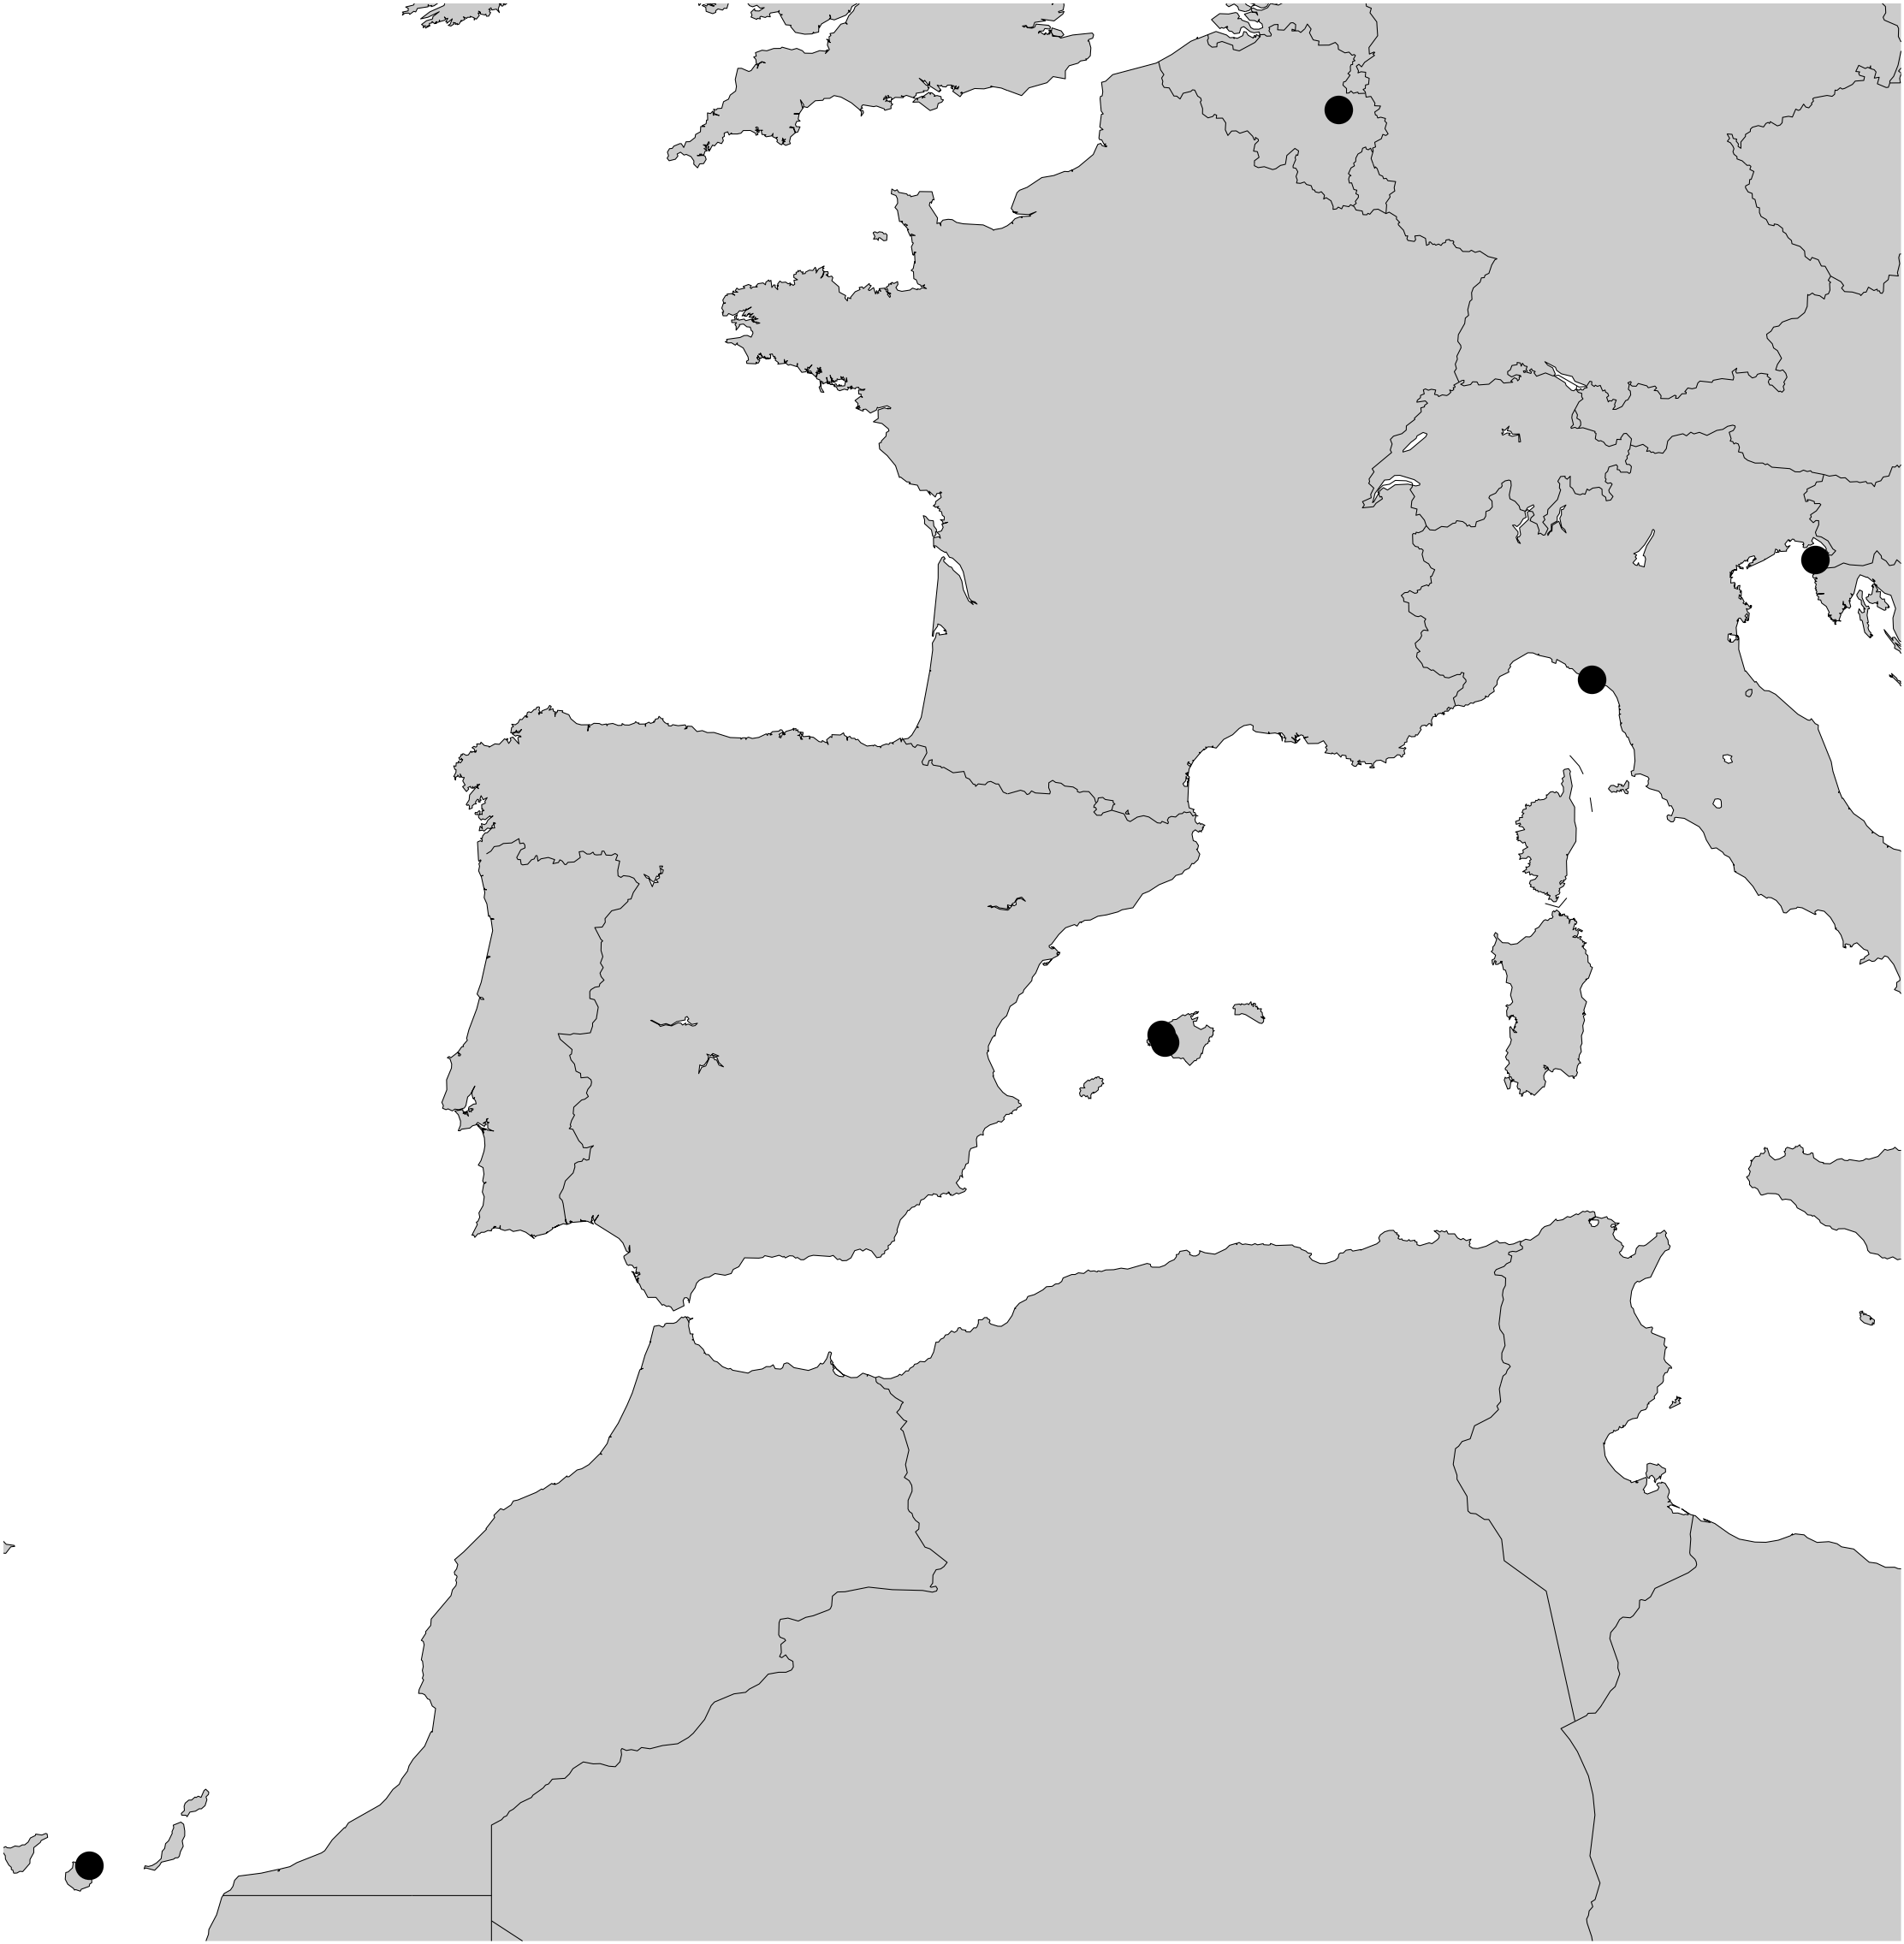
\includegraphics[width=.3\textwidth]{employment_map.png}};
    \begin{scope}[x={(image.south east)},y={(image.north west)}]
%    \draw[help lines,xstep=.1,ystep=.1] (0,0) grid (1,1);
%    \foreach \x in {0,1,...,9} { \node [anchor=north] at (\x/10,0) {0.\x}; }
%    \foreach \y in {0,1,...,9} { \node [anchor=east] at (0,\y/10) {0.\y}; }
    \node [anchor=west,text width=.65\textwidth,minimum height=1cm] (n2017) at (1.1,.95){2017/01--present\dotfill \textbf{Post-doctoral researcher \faAt~\href{http://labos.ulg.ac.be/gher/}{GHER} (ULiège)}\\ \textit{Deployment of a data interpolation tool in a Virtual Research Environment}};
    \node [anchor=west,text width=.65\textwidth,minimum height=1cm] (n2014) at (1.1,0.75){2014/03--2017/01\dotfill \textbf{Head of the Data Centre Facility \faAt~\href{www.socib.es}{\mbox{SOCIB}}}\\ \textit{Acquisition, processing and visualisation of oceanographic data}};
    \node [anchor=west,text width=.65\textwidth,minimum height=1cm] (n2013) at (1.1,0.55){2013/03--2014/03\dotfill \textbf{Post-doctoral researcher \faAt~\href{http://imedea.uib-csic.es/}{IMEDEA}}\\ \textit{Analysis of in situ, satellite altimetry and high-frequency radar data}};
    \node [anchor=west,text width=.65\textwidth,minimum height=1cm] (n2010) at (1.1,0.35){2010/10--2013/02\dotfill \textbf{Research assistant \faAt~\href{www.ulg.ac.be}{ULiège}}\\ \textit{Multivariate reconstruction of incomplete satellite images in the North Se}a};
    \node [anchor=west,text width=.65\textwidth,minimum height=1cm] (n2006) at (1.1,0.15){2006/10--2010/09 \dotfill \textbf{PhD Candidate \faAt~FRIA-FNRS}\\ \textit{Study of the Cape Ghir filament using numerical modeling and data interpolation}};
    
   	\node (liege) at (0.8,0.95) {};
   	\node (ulpgc) at (0.04,0.04) {};
   	\node (nurc) at (.95, .65) {};
   	\node (socib) at (.69, .47) {};
   	\node (imedea) at (.69, .47) {};

    \draw [{Circle[]}-,line width=1pt, color1, anchor=south] (n2017) to [out=180, in=0] (liege);
    \draw [{Circle[]}-,line width=1pt, color1, anchor=south] (n2014) to [out=180, in=0] (socib);
    \draw [{Circle[]}-,line width=1pt, color1, anchor=south] (n2013) to [out=180, in=0] (imedea);
    \draw [{Circle[]}-,line width=1pt, color1, anchor=south] (n2010) to [out=180, in=-45] (liege);
    \draw [{Circle[]}-,line width=1pt, color1, anchor=south] (n2006) to [out=180, in=-90] (liege);
    \draw [{Circle[]}-,line width=1pt, color1, anchor=south] (n2006) to [out=180, in=0] (ulpgc);
    \draw [{Circle[]}-,line width=1pt, color1, anchor=south] (n2006) to [out=180, in=-40] (nurc);
    \end{scope}
\end{tikzpicture}

\subsection*{Education}

\vspace*{-.5cm}

\parbox{.52\textwidth}{
\begin{chronology}[2]{2000}{2012}{.5\textwidth}[\textwidth]
\event[\decimaldate{15}{9}{2000}]{\decimaldate{30}{6}{2005}}{\parbox{2.5cm}{\large Engineer\\ in Physics}}
\event[\decimaldate{1}{9}{2005}]{\decimaldate{15}{9}{2006}}{\parbox{2.5cm}{\large D.E.A. in\\ Oceanography\\ (modelling)}}
\event[\decimaldate{1}{10}{2006}]{\decimaldate{15}{9}{2011}}{\parbox{3cm}{\large PhD in Sciences\\ (Oceanography)}}
\end{chronology}
}\parbox{.15\textwidth}{
~\\
Engineering\\
Fluid mechanics\\
Aerodynamics
}\parbox{.24\textwidth}{
~\\
Finite-element method\\
Numerical simulations\\
High-performance computing
}

\subsection*{Technical skills}

\parbox{.26\textwidth}{
\textbf{Programming}\\
Functional programming 				\\ 
Object oriented programming		\\
Test-oriented development			\\
Control version system (git, svn)	\\
Jupyter-notebooks					\\
Unit tests							\\	
%Data formats (json, csv, gpx, shapefiles)\\
}\parbox{.7\textwidth}{
\ganttset{bar height=.3}
\begin{ganttchart}[
	canvas/.style={fill=white},
    hgrid style/.style={draw=black!5, line width=.75pt},
    vgrid={*1{draw=CVorange, line width=.75pt, dashed},*2{draw=CVgrey, line width=.75pt, dashed}},
    title/.style={draw=none, fill=none},
    title label font=\bfseries,
    title label node/.append style={below=7pt},
    include title in canvas=false,
    bar label font=\mdseries\small\color{black!70},
    bar label node/.append style={left=.2cm},
    bar/.append style={draw=none, fill=black!63},
    bar incomplete/.append style={fill=black!70},
    bar progress label font=\mdseries\footnotesize\color{black!70},
    bar progress label node /.style=east,
    y unit chart=.5cm,
    progress=today,
    today=1,
    today label={}, 
    today rule /.style={draw=CVorange, line width=.75pt, dashed},
    progress label text = ,
    ]{1}{14}
   \gantttitle[title label node/.append style={below left=5pt and -3pt}]{Languages\quad}{0}
  %\gantttitle[title/.style={draw=CVorange,below=7pt}]{Languages}{0}
  \gantttitlelist[title/.style={draw=none, inner color=CVgrey,below=7pt}]{2006,2009,...,2019}{3} \\
  \ganttbar[name=bash, progress label text={awk, cron, git, ssh, ncftp, \ldots}]{Bash}{1}{14} \\
  \ganttbar[name=fortran,progress label text={data I/O, format conversion, optimisation}]{Fortran}{1}{14} \\
  \ganttbar[name=matlab,progress label text={\hspace{3.5cm}geostatistics, plotting, neural networks}]{MATLAB}{1}{7} \\
  \ganttbar[name=python,progress label text={matplotlib, numpy, scipy, pandas, virtualenv, \ldots}]{Python}{8}{14} \\
  \ganttbar[name=julia,progress label text={DataArrays, PyPlot, module developments}]{Julia}{11}{14} \\
  \ganttbar[name=javascript,progress label text={Leaflet, Highcharts, D3, Angular}]{Javascript}{11}{14}
\end{ganttchart}
}

\noindent \textbf{Web} HTML, CSS, markdown, javascript, Jekyll, wordpress, Dokuwiki, Mediawiki

\subsection*{Data analytics}

\skillbox{Spatial interpolation} \skillbox{Geostatistics} \skillbox{Big data} \skillbox{Predictive modelling} \skillbox{Cloud computing} \skillbox{Neural networks}\\
\skillbox{Signal processing} \skillbox{Open data} \skillbox{OGC standards} 


\subsection*{Soft skills}
\textbf{Project management:} Planning and monitoring \sepa scientific and technical reporting \sepa specification documents and strategic plans \sepa team leading, recruitment \sepa applications for grants and supports \sepa lean and agile management\\
\textbf{Communication:} Presentations at international conferences (English, Spanish, French) $\cdot$~ design of posters and leaflets (Darktable, GIMP, ImageMagick, Inkscape) $\cdot$~ social networks \sepa scienfic outreach\\ 
\textbf{Organisation:} International scientific meetings (~200 participants from 40 countries) $\cdot$~ software training workshops\\
\begin{tabularx}{\textwidth}{@{}lrlrlrlr @{}}
\textbf{Languages }	& \dotfill	 	& English 	& \threestar 	& Catalan 	& \twostar	& Italian	& \onestar\\
French (native)		& \fourstar 	& Spanish	& \threestar	& German	& \onestar	& Dutch 	& \halfstar	\\			
\end{tabularx}

\subsubsection*{Personal interests}
%---------------------------

\begin{tabular}{rlrlrlrl}
\faCameraRetro	& Photography & \faMapSigns & Ultra and mountain running 		& \faMapMarker & OpenStreetMap editing	& \faWordpress &Travel blogging \\
\Bicycle		& Road cycling& \faCloud 	 & Weather observation \& forecast	& \Industry    & UrbEx 					& & Coaching  			\\
\end{tabular}
%\textcolor{white}{Last modified: \today}
	

\end{document}